\documentclass{article}

\usepackage[a4paper, total={6in, 8in}]{geometry}
\usepackage[utf8]{inputenc}
\usepackage{fancyhdr}
\usepackage{graphicx}
\usepackage{enumitem}

\pagestyle{fancy}
\fancyhf{}
\lhead{John J Li}
\rhead{CSE360 Summer 2021 Assignment 2}
\rfoot{\thepage}
\renewcommand{\headrulewidth}{0.4pt}

\setlength{\parskip}{1em}
\setlength\parindent{0px}
\title{CSE360 Summer 2021 Assignment 2}
\date{\today}
\author{John J Li}

\begin{document}
    \maketitle
    \thispagestyle{empty}
    \noindent\rule{\textwidth}{0.8pt}

    An online music playlist system can have users that can do the following:
    \begin{itemize}
        \item 
        The user can add a song to the playlist. The system will ask the user to input the song
        name before searching for it in the system’s database.
        \begin{itemize}
            \item 
            If the song was not found, the system will add the song to a list that
            administrators use to know what songs should be added to the system’s
            database.
        \end{itemize}
        \item
        The user can play a song in the playlist. The system will ask the user to input the song
        name before searching for it in the user’s playlist.
        \item
        The user can remove a song from the playlist. The system will ask the user to input the
        song name before searching for it in the user’s playlist.
    \end{itemize}

    The system also has administrators that can do the following:
    \begin{itemize}
        \item 
        An administrator can do everything that a regular user can do.
        \item
        An administrator can add a song to the system’s database. The system will show the list
        of songs that users have been requesting.
        \item
        You can assume there is no limit to the number of songs that can be in the playlist or in the
        system’s database.
    \end{itemize}

    %###################################################################################

    \section*{Problem 1}

    Below are some user stories that describe some of the actions that
    users/administrators can do with the online music playlist system described
    above. Fill in the missing “???” parts so the user stories will match the
    description above.

    \begin{enumerate}[label=\quad\quad, leftmargin=*]
        \item
        As a “???”, I want to add a song to my playlist, so that I can listen to more songs.
        \item
        As a user, I want to “???”, so that I can listen to the song.
        \item
        As a user, I want to “???”, because I do not want to listen to the song anymore.
        \item
        As an administrator, I want to “???”, so that “???”.
    \end{enumerate}

    \subsection*{Solution}

    \begin{enumerate}[label=\quad\quad, leftmargin=*]
        \item
        As a user, I want to add a song to my playlist, so that I can listen to more songs.
        \item
        As a user, I want to play a song in my playlist, so that I can listen to the song.
        \item
        As a user, I want to remove a song from the playlist, because I do not want to listen to the song anymore.
        \item
        As an administrator, I want to add a new song to the system's database, 
        so that the users are satisfied with user-requested songs.
    \end{enumerate}


    %###################################################################################

    \section*{Problem 2}

    Below is a UML use case diagram that describes some of the interactions that a
    user may have with the system and how the system handles each action. Fill in
    the five missing “???” parts to make the diagram match the above problem
    description.

    \begin{center}
        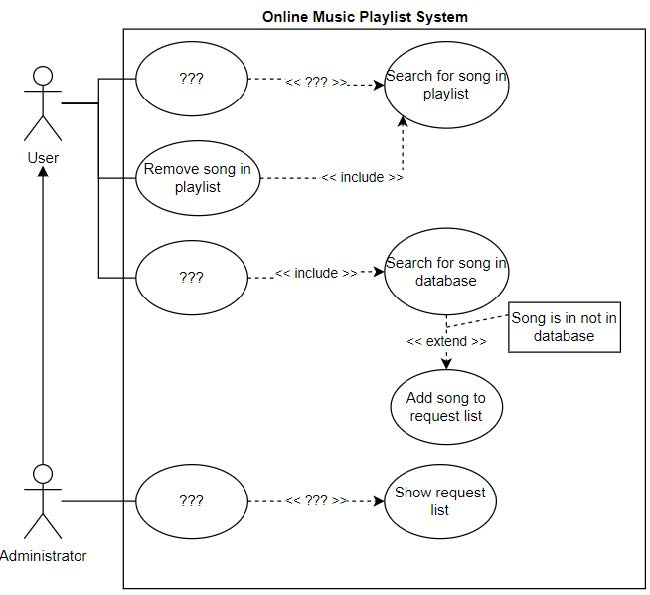
\includegraphics[scale=0.6]{Exercise 02_ Practice Problems.jpg}
    \end{center}

    \subsection*{Solution}

    \begin{center}
        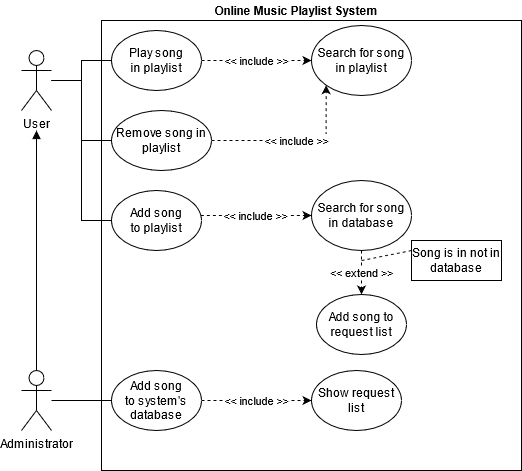
\includegraphics[scale=0.53]{Problem2.png}
    \end{center}

    %###################################################################################

    Let’s add some new features to the online music playlist system, downvoting a song and
    removing a song from the database.
    \begin{itemize}
        \item 
        A user can downvote a song. The system will add the song to a list that administrators
        use to know what songs should be removed from the system’s database.
        \item
        An administrator can remove a song from the system’s database. The system will show
        the list of songs that users have been downvoting.
    \end{itemize}

    %###################################################################################

    \section*{Problem 3}

    Write the user stories that describe the features that need to be added to the
    system.

    \subsection*{Solution}

    \begin{enumerate}[label=\quad\quad, leftmargin=*]
        \item
        As a user, I want to downvote a song, so that I can show others I dislike the song.
        \item
        As an administrator, I want to remove a song from the system's database, so that 
        the system's database will not be cluttered with songs that users dislike.
    \end{enumerate}

    %###################################################################################

    \section*{Problem 4}

    Modify the UML use case diagram from problem 2 to include the new interactions.

    \subsection*{Solution}

    \begin{center}
        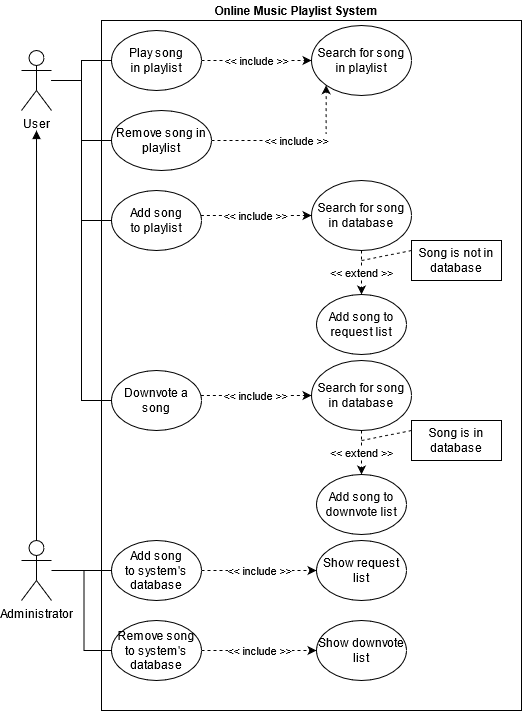
\includegraphics[scale=0.53]{Exercise02_Problem2.png}
    \end{center}

\end{document}